\documentclass[10pt]{beamer}

% %%% Style %%%
\mode<presentation>
{
  \usetheme{Berlin}
  \setbeamertemplate{blocks}[rounded]
  \setbeamercolor{block title}{bg=gray}
  \setbeamercovered{transparent}
}

% %%% Packages %%%
% Babel and fonts
\usepackage[english]{babel}
\usepackage[utf8]{inputenc}

% Graphics and images
\usepackage{xcolor}
\usepackage{graphicx}
\DeclareGraphicsExtensions{.pdf,.png,.jpg, .eps}
\usepackage{relsize}
\usepackage{colortbl}


% Math notation and symbols
\usepackage{mathrsfs}
\usepackage{amsthm}
\usepackage{bbold}
\usepackage{amsfonts}
\usepackage{amsmath}
\usepackage{amssymb}
% \usepackage{algorithm}
\usepackage{algpseudocode}
\usepackage{listings}

% \DeclareMathOperator*{\len}{\text{length of }}
% Backup slides
\usepackage{appendixnumberbeamer}

% Tables, Colums and the like
\usepackage{longtable}
\usepackage{listings}

% Hyperref
\usepackage{hyperref} 

% Boxes
\usepackage{fancybox}
\usepackage{lmodern}
\usepackage{tikz}
\usepackage{tcolorbox}
\usepackage{mdframed}	

\usepackage{hyperref}
\usepackage{listings}
\usepackage{setspace}
\usepackage{subfiles}
\usepackage{alltt}
\usepackage{mathtools}
\usepackage{fancyvrb}
\usepackage{url}

\usepackage{tikz}
\usetikzlibrary{shapes,arrows,positioning,calc}

\usepackage{xparse}
\usepackage{ifthen}
\usepackage{twoopt}

% Custom packages (needs absolute path from root document
%  Usage: \usepackage{appendixnumberbeamer}
%  Custom title page

\makeatletter

\setbeamertemplate{footline}
{
  \leavevmode%
  \hbox{%
  \begin{beamercolorbox}[wd=0.25\paperwidth,ht=2.25ex,dp=1ex,center]{author in head/foot}%
    \usebeamerfont{author in head/foot}\insertshortauthor
  \end{beamercolorbox}%
  \begin{beamercolorbox}[wd=0.50\paperwidth,ht=2.25ex,dp=1ex,center]{title in head/foot}%
    \usebeamerfont{title in head/foot}\inserttitle
  \end{beamercolorbox}%
  \begin{beamercolorbox}[wd=0.25\paperwidth,ht=2.25ex,dp=1ex,right]{date in head/foot}%
    \insertframenumber{} / \inserttotalframenumber\hspace*{2ex} 
  \end{beamercolorbox}}%
  \vskip0pt%
}
\makeatother

\makeatletter
\setbeamertemplate{headline}
{
  \leavevmode%
  \hbox{%
  \begin{beamercolorbox}[wd=\paperwidth,ht=2.25ex,dp=1ex,center]{title in head/foot}%
  \end{beamercolorbox}%
  }%
  \vskip0pt%
}
\makeatother

\defbeamertemplate*{title page}{customized}[1][]
{
  \begin{center}
    \begin{variableblock}{}{}{bg=blue}
      \begin{center}
	\usebeamerfont{title}\inserttitle\par
      \end{center}
    \end{variableblock}
  \end{center}

  \begin{center}
    \begin{minipage}{1.0\textwidth}
      \begin{center}
	\insertauthor

	\begin{scriptsize}
	  \insertdate
	\end{scriptsize}

      \end{center}
    \end{minipage}
  \end{center}
}

\input{includes/appendixnumberbeamer.sty}

% %%% Macros and custom commands %%%
\DeclareMathOperator*{\len}{\textbf{length of }}

\newcommand{\btVFill}{\vskip0pt plus 1filll}

\setbeamercolor{structure}{fg=cyan!90!black}

\newenvironment{variableblock}[3]{%
\setbeamercolor{block body}{#2}
\setbeamercolor{block title}{#3}
\begin{block}{#1}}{\end{block}}

\lstdefinestyle{JavaPlain}{ %
basicstyle=\scriptsize\ttfamily, % the size of the fonts 
numbers=left,                   % where to put the line-numbers
numberstyle=\tiny,      % the size of the fonts that are used for th
stepnumber=1,                   % the step between two line-numbers
numbersep=5pt,                  % how far the line-numbers are from the code
backgroundcolor=\color{white},  % choose the background color
showspaces=false,               % show spaces adding particular underscores
showstringspaces=false,         % underline spaces within strings
showtabs=false,                 % show tabs within strings adding 
frame=single,           % adds a frame around the code
tabsize=2,          % sets default tabsize to 2 spaces
captionpos=b,           % sets the caption-position to bottom
breaklines=true,        % sets automatic line breaking
breakatwhitespace=false,    % sets if automatic breaks should only happen
fancyvrb=true,
fvcmdparams=textbf 1 textit 1,
}

% Colors
\definecolor{ballblue}{rgb}{0.13, 0.67, 0.8}
\definecolor{brown(web)}{rgb}{0.65, 0.16, 0.16}
\definecolor{brown(traditional)}{rgb}{0.59, 0.29, 0.0}
\definecolor{amber}{rgb}{1.0, 0.75, 0.0}

\newcommand\Red[1]{\textcolor{red}{#1}}
\newcommand\Green[1]{\textcolor{green!50!black}{#1}}
\newcommand\LightGreen[1]{\textcolor{green!60!black}{#1}}
\newcommand\Blue[1]{\textcolor{blue!60!white}{#1}}
\newcommand\Violet[1]{\textcolor{violet}{#1}}
\newcommand\LightBlue[1]{\textcolor{ballblue}{#1}}
\newcommand\DarkBlue[1]{\textcolor{blue!60!black}{#1}}
\newcommand\Grey[1]{\textcolor{gray}{#1}}
\newcommand\Gray[1]{\textcolor{gray}{#1}}
\newcommand\Brown[1]{\textcolor{brown(web)}{#1}}
\newcommand\LightBrown[1]{\textcolor{brown(traditional)}{#1}}
\newcommand\Yellow[1]{\textcolor{amber}{#1}}

\newenvironment{redtext}{\color{red}}{\ignorespacesafterend}

% Helpers
\newcommand\Jcomment[1]{\LightGreen{// #1}}
\newcommand\JcommentMulti[1]{\LightGreen{/* #1}}
\newcommand\String[1]{\textcolor{blue!80!blue}{#1}}
\newcommand\Word[1]{\textcolor{purple!90!red}{#1}}
\newcommand\bang{!}
\newcommand\pipe{\|}

% Prints
% \newcommand\Jprintf[2][]{\LightBlue{printf}(\String{#1}, #2)}
\newcommandtwoopt{\Jprintf}[2][-NoValue-][-NoValue-]{%
    \ifthenelse{\equal{#2}{-NoValue-}}{\LightBlue{printf}(\String{#1})}{\LightBlue{printf}(\String{#1}, #2)}%
}

\newcommand\Jprintln[1]{\LightBlue{println}(\String{#1})}
\newcommand\JprintLN{\LightBlue{println}}

\newcommand\Jprint[1]{\LightBlue{print}(\String{#1})}
\newcommand\JPrint{\LightBlue{print}}

% Control structures
% Shortcut for JavaFor:
% \JavaFor (\Blue!init| \Green!n <= Math.sqrt(numero);| \Violet!n++|)
\newcommand\JavaForColors[3]{\Blue{#1}; \Green{#2}; \Violet{#3}}

\newcommand\Jfor[1][-NoValue-]{%
  \ifthenelse{\equal{#1}{-NoValue-}}{\Word{for}}{\JavaForO[#1]}%
}

\newcommandtwoopt{\JavaForO}[3][-NoValue-][-NoValue-]{%
    \JavaForOptions{#1}{#2}{#3}%
}

\DeclareDocumentCommand\JavaForOptions{ ggg }{%
  \Word{for}\IfValueT{#1}{%
    (\JavaForColors{#1}{#2}{#3}) %
  }%
}

% Shortcut for JavaFor:
% \JavaFor (\Blue!init| \Green!n <= Math.sqrt(numero);| \Violet!n++|)
\newcommand\Jif[1][-NoValue-]{%
  \ifthenelse{\equal{#1}{-NoValue-}}{\Word{if}}{\Word{if} (\Green{#1})}%
}

% Shortcut for JavaWhile:
% \JavaWhile(\Blue!init| \Green!n <= Math.sqrt(numero);| \Violet!n++|)
\newcommand\Jwhile[1][-NoValue-]{%
  \ifthenelse{\equal{#1}{-NoValue-}}{\Word{while}}{\Word{while} (\Green{#1})}%
}

% Other reserved words
\newcommand\Jthis{\textbf{\Word{this}}}
\newcommand\Jstatic{\Word{static}}
\newcommand\Jpublic{\Word{public}}
\newcommand\Jprivate{\Word{private}}
\newcommand\Jprotected{\Word{protected}}
\newcommand\Jdouble{\Word{double}}
\newcommand\Jfloat{\Word{float}}
\newcommand\Jint{\Word{int}}
\newcommand\Jvoid{\Word{void}}
\newcommand\Jreturn{\Word{return}}
\newcommand\Jclass{\Word{class}}
\newcommand\Jargs{\LightBrown{args}}
\newcommand\Jimport{\Word{import}}
\newcommand\Jnew{\Word{new}}
\newcommand\JsystemIn{System.\DarkBlue{\textit{\textbf{in}}}}
\newcommand\Jthrows{\Word{throws}}
\newcommand\Jtry{\Word{try}}
\newcommand\Jcatch{\Word{catch}}

\newenvironment{JavaCodePlain}[1][]
  { \VerbatimEnvironment%
    \begin{Verbatim}[#1]}
  { \end{Verbatim}  } 

\algdef{SE}[DOWHILE]{Do}{DoWhile}{\algorithmicdo}[1]{\algorithmicwhile\ #1}%
\renewcommand{\algorithmicrequire}{\textbf{Input:}}
\renewcommand{\algorithmicensure}{\textbf{Output:}}

\title[Laboratorio di Informatica - Lezione 3]{Laboratorio di Informatica \\ Lezione 3}
\author[Cristian Consonni]{Cristian Consonni}
\date[12/10/2015]{12 ottobre 2015}
\institute[UniTN]{Università degli Studi di Trento}

% %%% Put slides with section name at the begining of each section %%%
\AtBeginSection[]
{
  \begin{frame}<beamer>
    \frametitle{Outline for section \thesection}
    \tableofcontents[currentsection]
  \end{frame}
}
\setbeamertemplate{navigation symbols}{}

\begin{document}

%%%%%%%%%% TITLE %%%%%%%%%%
% Formerly part of title.tex
\begin{frame}
  \titlepage
\end{frame}

\begin{frame}{Outline}
  \tableofcontents
\end{frame}
%%%%%%%%%% END TITLE %%%%%%%%%%

\begin{frame}{Chi sono}
  Cristian Consonni

  \begin{itemize}
    \item \textbf{DISI - Dipartimento di Ingegneria e Scienza dell'Informazione}
    \item \textbf{Pagina web} del laboratorio: \structure{\url{http://disi.unitn.it/~consonni/teaching}}
    \item \textbf{Email}: \structure{\url{cristian.consonni@unitn.it}}
    \item \textbf{Ufficio}: Povo 2 - Open Space 9
      \begin{itemize}
	\item Per domande: scrivetemi una mail
	\item Ricevimento: su appuntamento via mail
      \end{itemize}
  \end{itemize}
\end{frame}


\section{Procedure e funzioni}

\begin{frame}{Metodo della bisezione}

  Negli esercizi della scorsa volta abbiamo calcolato gli zeri di una \textbf{funzione}:
  \begin{equation}
    f(x) = x^3 - x - 2
  \end{equation}

\end{frame}


\begin{frame}[fragile]\frametitle{Funzioni (I)}

  Possiamo definire delle funzioni per rendere il codice:
  \begin{itemize}
    \item più \textbf{leggibile}
    \item più \textbf{riutilizzabile}
    \item più \textbf{compatto} e semplice da modificare
  \end{itemize}
\end{frame}

\begin{frame}[fragile]\frametitle{Funzioni (II)}

  Dichiarazione e implementazione di una funzione:

  \begin{JavaCodePlain}[commandchars=\\!|]
  \Jpublic \Jstatic \Jdouble f(\Jdouble x) {
      \Jreturn(x * x * x - x - 2);
  }
  \end{JavaCodePlain}     
  analizziamo la sintassi parola per parola.

\end{frame}

\begin{frame}[fragile]\frametitle{Funzioni (III)}

  Dichiarazione e implementazione di una funzione:
  
  \begin{JavaCodePlain}[commandchars=\\!|]
  \Red!public| \Red!static| \Grey!double f(double x) {|
      \Grey!return(x * x * x - x - 2);|
  \Grey!}|
  \end{JavaCodePlain}
  
  Le parole chiave \Red{public} e \Red{static} modificano la
  visibilità della funzione. Per ora ignoratele e scrivete
  sempre così.

\end{frame}


\begin{frame}[fragile]\frametitle{Funzioni (IV)}

  Dichiarazione e implementazione di una funzione:
  
  \begin{JavaCodePlain}[commandchars=\\!|]
  \Grey!public static| \Red!double| \Grey!f(double x) {|
      \Grey!return(x * x * x - x - 2);|
  \Grey!}|
  \end{JavaCodePlain}
  
  Questo è il \textbf{tipo del valore di ritorno} (\emph{return type})
  della funzione, vuol dire, in questo caso, che la funzione restituisce
  un double.

\end{frame}

\begin{frame}[fragile]\frametitle{Funzioni (V)}

  Dichiarazione e implementazione di una funzione:

  \begin{JavaCodePlain}[commandchars=\\!|]
  \Grey!public static| \Grey!double| \Red!f|\Grey!(double x) {|
      \Grey!return(x * x * x - x - 2);|
  \Grey!}|
  \end{JavaCodePlain}
  
  Dopo il tipo di ritorno si specifica il \textbf{nome} della funzione,
  come per le variabili si tratta dell'identificativo da utilizzare per
  utilizzare una funziona.

\end{frame}

\begin{frame}[fragile]\frametitle{Funzioni (VI)}

  Dichiarazione e implementazione di una funzione:

  \begin{JavaCodePlain}[commandchars=\\!|]
  \Grey!public static| \Grey!double| \Grey!f|\Red!(|\Grey!double x|\Red!)| \Grey!{|
      \Grey!return(x * x * x - x - 2);|
  \Grey!}|
  \end{JavaCodePlain}

  Le funzioni sono caratterizzate dalle parentesi tonde \texttt{f()} che servono
  per potere \emph{chiamare} una funzioone.

\end{frame}

\begin{frame}[fragile]\frametitle{Funzioni (VII)}

  Dichiarazione e implementazione di una funzione:

  \begin{JavaCodePlain}[commandchars=\\!|]
  \Grey!public static| \Grey!double| \Grey!f(|\Red!double x|) \Grey!{|
      \Grey!return(x * x * x - x - 2);|
  \Grey!}|
  \end{JavaCodePlain}

  All'interno delle parentesi tonde si indicano gli argometi della
  funzione detti \textbf{parametri formali}.

\end{frame}

\begin{frame}[fragile]\frametitle{Funzioni (VIII)}

  Dichiarazione e implementazione di una funzione:

  \begin{JavaCodePlain}[commandchars=\\!|]
  \Grey!public static| \Grey!double| \Grey!f(|\Red!double| \Grey!x) {|
      \Grey!return(x * x * x - x - 2);|
  \Grey!}|
  \end{JavaCodePlain}

  Ogni \emph{parametro formale} è caratterizzato da un proprio  \textbf{tipo}...

\end{frame}

\begin{frame}[fragile]\frametitle{Funzioni (IX)}

  Dichiarazione e implementazione di una funzione:

  \begin{JavaCodePlain}[commandchars=\\!|]
  \Grey!public static| \Grey!double| \Grey!f(double| \Red!x|\Grey!) {|
      \Grey!return(x * x * x - x - 2);|
  \Grey!}|
  \end{JavaCodePlain}

  e da un proprio \textbf{nome}.

\end{frame}

\begin{frame}[fragile]\frametitle{Funzioni (X)}

  Dichiarazione e implementazione di una funzione:

  \begin{JavaCodePlain}[commandchars=\\!|]
  \Grey!public static| \Grey!double| \Grey!f(|\Red!double x1, int x2|\Grey!) {|
      \Grey!return(x1 * x1 * x1 - x2 - 2);|
  \Grey!}|
  \end{JavaCodePlain}

  Una funzione può avere più parametri formali ciascuno caratterizzato dal
  proprio tipo e nome.

\end{frame}

\begin{frame}[fragile]\frametitle{Funzioni (XI)}

  Dichiarazione e implementazione di una funzione:
  
  \begin{JavaCodePlain}[commandchars=\\!|]
  \Grey!public static double f(double x) |\Red!{|
      \Red!return(x * x * x - x - 2);|
  \Red!}|
  \end{JavaCodePlain}

  Le parentesi graffe \texttt{\{\}} delimitano il \textbf{corpo}
  (o \emph{scope}) della funzione.

\end{frame}

\begin{frame}[fragile]\frametitle{Funzioni (XII)}

  Dichiarazione e implementazione di una funzione:
  \begin{JavaCodePlain}[commandchars=\\!|]
  \Grey!public static double f(double x) {|
      \Red!return|\Grey!(x * x * x - x - 2);|
  \Grey!}|
  \end{JavaCodePlain}

  La parola riservata \Red{return} indica quale valore sarà restituito dalla funzione.

\end{frame}

\begin{frame}[fragile]\frametitle{Funzioni: riassumendo}

  Dichiarazione e implementazione di una funzione:
  \begin{JavaCodePlain}[commandchars=\\!|]
  \Red!public static| \Green!double| \Violet!f|(\Blue!double x|) {
      \Brown!return|(x * x * x - x - 2);
  }
  \end{JavaCodePlain}

  \begin{itemize}
   \item \Red{\texttt{public static} $\rightarrow$ visibilità}
   \item \Green{\texttt{double} $\rightarrow$ tipo del valore di ritorno}
   \item \Violet{\texttt{f} $\rightarrow$ nome della funzione}
   \item \Blue{\texttt{double x} $\rightarrow$ parametri formali}
   \item \Brown{\texttt{return} $\rightarrow$ valore di ritorno}
  \end{itemize}

\end{frame}

\begin{frame}[fragile]\frametitle{Procedure}
  Le procedure sono funzioni che non restituiscono alcun valore.
  Per indicare questo fatto si usa come valore di ritorno \Word{\textbf{void}}:
  
  \begin{JavaCodePlain}[commandchars=\\!|]
  \Red!public static| \Green!\textbf!void|| \Violet!f|(\Blue!double x|) {
    \Jprintln!"Questa è una procedura"|;
  }
  \end{JavaCodePlain}
  {\scriptsize (Nelle slide userò \LightBlue{printf} e \LightBlue{println} invece di
   \LightBlue{System.out.printf} o \LightBlue{System.out.println}).}
 
  \begin{itemize}
   \item \Red{\texttt{public static} $\rightarrow$ visibilità}
   \item \Green{\textbf{\texttt{void}} $\rightarrow$ nessun valore ritornarto, è una \textbf{procedura}}
   \item \Violet{\texttt{f} $\rightarrow$ nome della procedura}
   \item \Blue{\texttt{double x} $\rightarrow$ parametri formali}
   \item \Brown{\texttt{return} $\rightarrow$ valore di ritorno}
  \end{itemize}
\end{frame}

\begin{frame}[fragile]\frametitle{Funzioni e procedure: esempio (I)}

  \begin{JavaCodePlain}[commandchars=\\!|]
  \Word!public class| FunzioniProcedure {

    \Jcomment!Questa è una funzione di due parametri x e y|
    \Jcomment!che restituisce un intero|
    \Word!public static int| somma(\Word!int| x, \Word!int| y) {
        \Word!return| x + y;
    }

    \dots
  \end{JavaCodePlain}


\end{frame}

\begin{frame}[fragile]\frametitle{Funzioni e procedure: esempio (II)}

  \begin{JavaCodePlain}[commandchars=\\!|]
    \dots

    \Jcomment!Questa è una procedura di due parametri x e y|
    \Word!public static void| stampaSomma(\Word!int| x, \Word!int| y) {

      \Jprintf["== Somma di due numeri ==\%n"];
      \Jprintf["Il primo parametro (x) vale \%d.\%n"][x];
      \Jprintf["Il secondo parametro (y) vale \%d.\%n"][y];
      \Jprintf["La somma di \%d e \%d è \%d.\%n"][x, y, x + y];

      \Jcomment!La riga seguente può essere omessa,|
      \Jcomment!io preferisco indicarla per chiarezza|
      \Word!return|;
    }
    
    \dots
  \end{JavaCodePlain}

\end{frame}

\begin{frame}[fragile]\frametitle{Funzioni e procedure: esempio (III)}

  \begin{JavaCodePlain}[commandchars=\\!|]
    \dots

    \Jcomment!Questo è il main, come al solito|
    \Word!public static void| main(String[] \LightBrown!args|) {
    
      \Jint a = 7;
      \Jint b = 11;
      \Jint risultato;
      
      \Jcomment!Chiamata della funzione|
      risultato = somma(a, b);
      \Jprintf["risultato: \%d.\%n"][risultato];
      
      \Jcomment!Chiamata della procedura|
      stampaSomma(a, b);
    }
  }
  \end{JavaCodePlain}

\end{frame}

\begin{frame}[fragile]\frametitle{Parametri attuali}

  Nella slide precedente abbiamo visto
  \begin{JavaCodePlain}[commandchars=\\!|]
  \Word!public static int| somma(\Word!int| x, \Word!int| y) {
  \dots
  \Word!public static void| stampaSomma(\Word!int| x, \Word!int| y) {
  \end{JavaCodePlain}
  \textbf{definizioni} della funzione \texttt{somma} e della procedura
  \texttt{stampaSomma}. Entrambe le definizioni hanno come \textbf{parametri formali} 
  le variabli \texttt{x} e \texttt{y}.\newline
  
  Le chiamate:
  \begin{JavaCodePlain}[commandchars=\\!|]
  risultato = somma(x, y);
  \dots
  stampaSomma(x, y);
  \end{JavaCodePlain}
  hanno come \textbf{parametri attuali} le variabli \texttt{a} e \texttt{b}.

\end{frame}

\begin{frame}[fragile]\frametitle{Parametri passati per valore (I)}

  \begin{JavaCodePlain}[commandchars=\\!|]
  \Jpublic \Jclass StampaParola {

    \Jcomment!di solito in Java si usa il CamelCase|
    \Jpublic \Jstatic \Jvoid stampaParolaInVerticale(String parola) {

      \Jcomment!String.toUpperCase() rende una stringa tutta|
      \Jcomment!maiuscola|
      parola = parola.toUpperCase();
      
      \Jcomment!String.length restituisce la lunghezza della parola|
      for(int i = 0; i < parola.length(); i++) {

	      \Jcomment!parola.charAt(i) restituisce l'i-esimo carattere|
	      \Jcomment!della parola si parte a contare da zero.|
	      \JprintLN(parola.charAt(i));
      }
    }
  \dots
  \end{JavaCodePlain}

\end{frame}

\begin{frame}[fragile]\frametitle{Parametri passati per valore (II)}

  \begin{JavaCodePlain}[commandchars=\\!|]
   \dots

    \Jpublic \Jstatic \Jvoid main(String[] args) {
    
      String parola = \String!"Ciao"|;
      
      \Jprintf["La parola da stampare è: \%s.\%n"][parola];
      stampaParolaInVerticale(parola);
      \Jprintf["La parola stampata è: \%s.\%n"][parola];

    }
  }
  \end{JavaCodePlain}

\end{frame}

\begin{frame}[fragile]\frametitle{Funzioni: diagramma}

%   \begin{tikzpicture}[node distance=.3\textwidth]
%     \node (x)  {$x$};
%     \node (y) [right of=x] {$y=f(x)$};
%     \draw[->,thick] (x) -- node[above] {$f$} (y);
%   \end{tikzpicture}

  Possiamo immaginare una funzione come una ``scatola nera'' che
  rende in ingresso i parametri e restituisce un valore:

  \begin{center}
    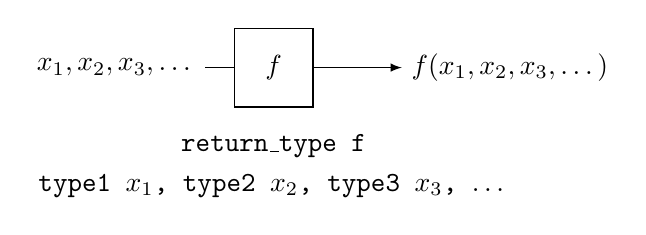
\begin{tikzpicture}[baseline=-0.5ex, on grid, node distance=2cm]
      \node (init) {$x_1, x_2, x_3, \dots$};
      \node[draw,right of=init, minimum size=1cm] (func) {$f$}; 
      \node[right= 3cm of func] (end) {$f(x_1, x_2, x_3, \dots)$};
      \node[below= 1cm of func] (def1) {\texttt{return\_type f}};
      \node[below= 0.5cm of def1] (def2) {\texttt{type1 $x_1$, type2 $x_2$, type3 $x_3$, $\dots$}};
      \draw[-] (init)--(func);
      \draw[-latex] (func)--(end);
    \end{tikzpicture}
  \end{center}
  
  \pause{
  \begin{alertblock}{Attenzione}
    In un linguaggio imperativo è possibile che una funzioni modifichi il valore di alcune variabili in ingresso!
  \end{alertblock}
  }

\end{frame}


\section{Iterazione e ricorsione}
\begin{frame}{Iterazione e ricorsione (I)}

  Una distizione importante per quanto riguarda le funzione è la
  seguente:
  \begin{itemize}
   \item funzioni \textbf{iterative}
   \item funzioni \textbf{ricorsive}
  \end{itemize}
  
  Una funzione \alert{\textbf{ricorsiva}} è una funzione che
  \textbf{richiama se stessa}. Altrimenti è \structure{\textbf{iterativa}}.

  Le funzioni viste finora sono iterative.
\end{frame}

\begin{frame}{Iterazione e ricorsione (II)}

  Le funzioni ricorsive si trovano molto comunemente anche in matematica.
  
  Esempi:
  \begin{itemize}
   \item fattoriale: $n! = n \cdot n - 1 \cdot \dots \cdot 3 \cdot 2 \cdot 1 := n \cdot (n - 1)!$
   \item successione di Fibonacci: $F_{n} = F_{n-1} + F_{n-2}$
  \end{itemize}
  ovviamente la definzione deve avere alcuni \textbf{casi limite} altrimenti si andrebbe
  avanti all'infinito.

  ${}$\newline

  \begin{minipage}{0.8\paperwidth}
    Per i casi di cui sopra:
    \begin{itemize}
      \item fattoriale: $n = 0 \Rightarrow 0! = 1$ (il fattoriale non è definito per numeri interi negativi)
      \item successione di Fibonacci: $F_{0} = 0$ e $F_{1} = 1$\footnote{Tradizionalmente si definiva 
	    $F_{0} = 1$ e $F_{1} = 1$, ma ora si definisce di solito come sopra. Si veda anche \url{https://oeis.org/A000045}}
    \end{itemize}
  \end{minipage}

\end{frame}

\begin{frame}[fragile]\frametitle{Definizione ricorsiva del fattoriale}

  \begin{JavaCodePlain}[commandchars=\\!|]
  \Jpublic \Jclass FattorialeRicorsivo {

    \Jpublic \Jstatic \Jint fattoriale(\Jint n) {
      \Jif[n == 0] {
        \Jreturn 1;
      }
      \Jreturn n * fattoriale(n - 1);
    }

    \Jpublic \Jstatic \Jvoid main(String[] \Jargs) {
      \Jint numero = 10;
      \Jint risultato = 0;
      
      risultato = fattoriale(numero);
      \Jprintf["Il fattoriale di \%d è: \%d"][numero, risultato];
    }
  }
  \end{JavaCodePlain}
\end{frame}

\section{Variabili globali e locali}

\begin{frame}[fragile]\frametitle{Variabili globali e locali}

  All'interno di una funzione possono essere definite nuove \emph{variabili}.
  Queste variabili sono \textbf{locali} ovvero esistono e sono utilizzatibili 
  solo all'interno della funzione stessa.
  
  \begin{JavaCodePlain}[commandchars=\\!|]
  \dots
  \Word!public static int| somma(\Word!int| x, \Word!int| y) {
      \Jint ris;
      ris = x + y;
      \Word!return| ris;
  }

  \Word!public static void| main(String[] \LightBrown!args|) {    
    \Jint a = 7;
    \Jint b = 11;
    \Jint risultato;
    
    \Jcomment!Qui *non posso* usare ris\bang|
    \dots 
  \end{JavaCodePlain}

\end{frame}

\begin{frame}[fragile]\frametitle{Variabili globali e locali}

  Le parentesi graffe \texttt{\{\}} definiscono uno \textbf{scope}
  (lett. \emph{ambito}) ovvero un blocco di codice.

  \begin{JavaCodePlain}[commandchars=\\!|]

  \Word!public static void| main(String[] \LightBrown!args|) {    
    \Jint fatt  = 1;
    \Jint N = 10;

    \Jfor (\Jint n = 2; n < N; n++) {
      \Jcomment!La variabile n esiste solo all'interno di questo|
      \Jcomment!blocco di codice|
      \dots
    }
  
  \end{JavaCodePlain}

\end{frame}

\begin{frame}[fragile]\frametitle{Variabili globali e locali}

  Come avete già visto potete usare variabili che avete definito
  in blocco più esterno dentro blocchi più interni.

  \begin{JavaCodePlain}[commandchars=\\!|]

  \Word!public static void| main(String[] \LightBrown!args|) {    
    \Jint fatt  = 1;
    \Jint N = 10;

    \Jfor (\Jint n = 2; n < N; n++) {
      \Jcomment!fatt è definita nel blocco più esterno, quindi|
      \Jcomment!la posso usare anche qui|
      fatt = fatt * n;
    }
  
  \end{JavaCodePlain}

\end{frame}

\begin{frame}[fragile]\frametitle{Variabili globali e locali}

  Posso definere delle variabili che possano essere usate in ogni
  scope, queste si dicono variabili \textbf{globali}.

  \begin{JavaCodePlain}[commandchars=\\!|]
  \Word!public class| GlobaliLocali {
    
    \Jint numero = 0;
    
  \dots
  \end{JavaCodePlain}

  queste variabili possono essere modificate da ogni funzione e quindi
  \alert{vanno usate con attenzione}. È meglio limitare il più possibile
  lo scope di una variabile.
    
  Cercate di dare nomi significativi alle variabili globali altrimenti
  sembra che ``piovano dal cielo''. Solitamente le variabili globali
  (specie se rappresentano una costante) si scrivono con nomi
  tutti in \texttt{MAIUSCOLO}.
  
\end{frame}

\section{Esericizi (parte I)}
\begin{frame}{Esercizi (parte I) (I)}

  Scrivere un programma in cui:
  \begin{itemize}
   \item si inserire un numero intero $N \leq 10$ da console;
   \item Inizializzare un  array  di  interi di lunghezza $N$ con  
   i valori presi in input  da  console (ciclare finché non si ottengono $N$ valori
   del tipo desiderato);
   \item Dopo aver letto tutti i valori stampare progressivamente i valori inseriti;
  \end{itemize}
\end{frame}
  
\begin{frame}[fragile]\frametitle{Esercizi (parte I) (II)}  
  Per esempio, se  l'array inserito è  il  seguente  $\{2,  5,  7,  4\}$. Il  programma deve ciclare
  sull’array stampando:
  \begin{center}
  \begin{JavaCodePlain}[commandchars=\\!|]
      2
      2, 5
      2, 5, 7
      2, 5, 7, 4
  \end{JavaCodePlain}   
  \end{center}

  \begin{itemize}
   \item Suggerimento: sono due  \Jfor{} annidati (uno all'interno dell’altro) utilizzate
   \texttt{System.out.}\JPrint{} per  stampare i valori e quando uscite dal \Jfor{}
   interno stampate una riga vuota
  \end{itemize}


\end{frame}


\section{Array}
% \begin{frame}{Array (I)}
% 
%   Supponiamo di volere avere delle variabili che contegano tutte
%   le lettere (minuscole) dell'alfabeto (\texttt{\Word{char}}).
% 
% 
%   Dovere gestire 26 variabili potrebbe essere complicato!
% 
% 
%   Possiamo usare un \textbf{array}. 
%   
% \end{frame}

  \begin{frame}{Array (I)}
  \begin{table}[]
  \centering
    \begin{tabular}{cccccccccc}
      \multicolumn{10}{c}{}                                                                                                                                                                                                                                                                                                                                                                                                                                                                     \\
      \rowcolor[HTML]{EFEFEF} 
      {\color[HTML]{FE0000} \textbf{0}}               & \textbf{1}                                     & \textbf{2}                                     & \textbf{3}                                     & \textbf{4}                                     & \textbf{5}                                     & \textbf{6}                                     & \textbf{7}                                     & \textbf{8}                                     & \textbf{9}                                     \\ \hline
      \rowcolor[HTML]{9AFF99} 
      \multicolumn{1}{|c|}{\cellcolor[HTML]{9AFF99}\String{"a"}} & \multicolumn{1}{c|}{\cellcolor[HTML]{9AFF99}\String{"b"}} & \multicolumn{1}{c|}{\cellcolor[HTML]{9AFF99}\String{"c"}} & \multicolumn{1}{c|}{\cellcolor[HTML]{9AFF99}\String{"d"}} & \multicolumn{1}{c|}{\cellcolor[HTML]{9AFF99}\String{"e"}} & \multicolumn{1}{c|}{\cellcolor[HTML]{9AFF99}\String{"f"}} & \multicolumn{1}{c|}{\cellcolor[HTML]{9AFF99}\String{"g"}} & \multicolumn{1}{c|}{\cellcolor[HTML]{9AFF99}\String{"h"}} & \multicolumn{1}{c|}{\cellcolor[HTML]{9AFF99}\String{"i"}} & \multicolumn{1}{c|}{\cellcolor[HTML]{9AFF99}\String{"j"}} \\ \hline
      \multicolumn{10}{c}{}                                                                                                                                                                                                                                                                                                                                                                                                                                                      
    \end{tabular}
  \end{table}  
  
  Un \textbf{array} (o \textbf{vettore}) è una \emph{struttura dati} composto da un \textbf{numero finito} di 
  elementi tutti dello \textbf{stesso tipo}.

\end{frame}

\begin{frame}{Array (I)}
  
  Simili al concetto matematico di vettore:
  
  \begin{equation*}
    v = \left( \begin{array}{c}
                1 \\
                0 \\
                4 \\
                7 \\
               \end{array}\right)
  \end{equation*}

\end{frame}

\begin{frame}{Array (II)}
  \begin{enumerate}
   \item Dichiarazione di un array:
  \end{enumerate}
  \begin{center}
    \begin{columns}[T]
      \begin{column}[T]{3cm}
	\begin{itemize}
	 \item 	\texttt{\Violet{tipo} \Green{nome}\textbf{[]}}
	\end{itemize}
      \end{column}
      \begin{column}[T]{3cm}
	\begin{itemize}
	 \item \texttt{\Violet{tipo}\textbf{[]} \Green{nome}}
	\end{itemize}
      \end{column}
    \end{columns}   
  \end{center}

  \begin{enumerate}
    \setcounter{enumi}{1}
    \item Allocazione:
  \end{enumerate}
  \begin{itemize}
   \item \texttt{\Green{nome} = \Red{\textbf{new}} \Violet{tipo}[\Blue{dimensione}]}
  \end{itemize}

  \begin{enumerate}
    \setcounter{enumi}{2}
    \item Diachiarazione e inizializzazione con literals:
  \end{enumerate}
  \begin{itemize}
   \item \texttt{\Violet{tipo}\textbf{[]} \Green{nome} =\textbf{\{}val1, val2, ...\textbf{\}}} 
  \end{itemize}

\end{frame}

\begin{frame}[fragile]\frametitle{Array (III)}

  \begin{JavaCodePlain}[commandchars=\\!|]
  \Jpublic \Jclass Array {

    \Jpublic \Jstatic \Jvoid main(String[] args) {
    
      \Jint[] vettore;      
      vettore = \Word!new| int[10];

    \dots
  \end{JavaCodePlain}

\end{frame}

\begin{frame}{Array (IV)}
  \begin{table}[]
    \centering
    \begin{tabular}{cccccccccc}
      \multicolumn{10}{c}{\textbf{indici}}                                                                                                                                                                                                                                                                                                                                                                                                                                                                     \\
      \rowcolor[HTML]{EFEFEF} 
      {\color[HTML]{FE0000} \textbf{0}}               & \textbf{1}                                     & \textbf{2}                                     & \textbf{3}                                     & \textbf{4}                                     & \textbf{5}                                     & \textbf{6}                                     & \textbf{7}                                     & \textbf{8}                                     & \textbf{9}                                     \\ \hline
      \rowcolor[HTML]{9AFF99} 
      \multicolumn{1}{|c|}{\cellcolor[HTML]{9AFF99}\String{"a"}} & \multicolumn{1}{c|}{\cellcolor[HTML]{9AFF99}\String{"b"}} & \multicolumn{1}{c|}{\cellcolor[HTML]{9AFF99}\String{"c"}} & \multicolumn{1}{c|}{\cellcolor[HTML]{9AFF99}\String{"d"}} & \multicolumn{1}{c|}{\cellcolor[HTML]{9AFF99}\String{"e"}} & \multicolumn{1}{c|}{\cellcolor[HTML]{9AFF99}\String{"f"}} & \multicolumn{1}{c|}{\cellcolor[HTML]{9AFF99}\String{"g"}} & \multicolumn{1}{c|}{\cellcolor[HTML]{9AFF99}\String{"h"}} & \multicolumn{1}{c|}{\cellcolor[HTML]{9AFF99}\String{"i"}} & \multicolumn{1}{c|}{\cellcolor[HTML]{9AFF99}\String{"j"}} \\ \hline
      \multicolumn{10}{c}{{\color[HTML]{009901} valori}}                                                                                                                                                                                                                                                                                                                                                                                                                                                      
    \end{tabular}
  \end{table}
  
  Per accedere all'elemento con indice \texttt{\Blue{i}} dell'array si usa la sintassi:
  \begin{center}
    \texttt{\Green{nome}\textbf{[}\Blue{i}\textbf{]}}
  \end{center}
  
  Notate che:
  \begin{itemize}
   \item gli indici partono da \alert{\textbf{zero}} e arrivono fino alla \structure{\textbf{lunghezza dell'array meno uno}}
   \item il primo elemento è accessibile con \texttt{\Green{nome}\textbf{[}\Blue{0}\textbf{]}}
   \item l'ultimo elemento è accessibile con \texttt{\Green{nome}\textbf{[}\Blue{len - 1}\textbf{]}} (dove \texttt{len}
	 è la lunghezza dell'array.
  \end{itemize}

\end{frame}

\begin{frame}{Array (V)}
  \begin{table}[]
    \centering
    \begin{tabular}{cccccccccc}
      \multicolumn{10}{c}{\textbf{indici}}                                                                                                                                                                                                                                                                                                                                                                                                                                                                     \\
      \rowcolor[HTML]{EFEFEF} 
      {\color[HTML]{FE0000} \textbf{0}}               & \textbf{1}                                     & \textbf{2}                                     & \textbf{3}                                     & \textbf{4}                                     & \textbf{5}                                     & \textbf{6}                                     & \textbf{7}                                     & \textbf{8}                                     & \textbf{9}                                     \\ \hline
      \rowcolor[HTML]{9AFF99} 
      \multicolumn{1}{|c|}{\cellcolor[HTML]{9AFF99}\String{"a"}} & \multicolumn{1}{c|}{\cellcolor[HTML]{9AFF99}\String{"b"}} & \multicolumn{1}{c|}{\cellcolor[HTML]{9AFF99}\String{"c"}} & \multicolumn{1}{c|}{\cellcolor[HTML]{9AFF99}\String{"d"}} & \multicolumn{1}{c|}{\cellcolor[HTML]{9AFF99}\String{"e"}} & \multicolumn{1}{c|}{\cellcolor[HTML]{9AFF99}\String{"f"}} & \multicolumn{1}{c|}{\cellcolor[HTML]{9AFF99}\String{"g"}} & \multicolumn{1}{c|}{\cellcolor[HTML]{9AFF99}\String{"h"}} & \multicolumn{1}{c|}{\cellcolor[HTML]{9AFF99}\String{"i"}} & \multicolumn{1}{c|}{\cellcolor[HTML]{9AFF99}\String{"j"}} \\ \hline
      \multicolumn{10}{c}{{\color[HTML]{009901} valori}}                                                                                                                                                                                                                                                                                                                                                                                                                                                      
    \end{tabular}
  \end{table}
  
  Per accedere all'elemento con indice \texttt{\Blue{i}} dell'array si usa la sintassi:
  \begin{center}
    \texttt{valore = \Green{nome}\textbf{[}\Blue{i}\textbf{]}}
  \end{center}
  
  Esempi:
  \begin{itemize}
   \item \texttt{\Green{nome}\textbf{[}\Blue{0}\textbf{]}} $\rightarrow$ \String{"a"}
   \item \texttt{\Green{nome}\textbf{[}\Blue{4}\textbf{]}} $\rightarrow$ \String{"e"}
   \item \texttt{\Green{nome}\textbf{[}\Blue{10}\textbf{]}} $\rightarrow$ \alert{\textbf{Errore: out of range}}
  \end{itemize}

\end{frame}

\begin{frame}{Array (VI)}
  \begin{table}[]
    \centering
    \begin{tabular}{cccccccccc}
      \multicolumn{10}{c}{\textbf{indici}}                                                                                                                                                                                                                                                                                                                                                                                                                                                                     \\
      \rowcolor[HTML]{EFEFEF} 
      {\color[HTML]{FE0000} \textbf{0}}               & \textbf{1}                                     & \textbf{2}                                     & \textbf{3}                                     & \textbf{4}                                     & \textbf{5}                                     & \textbf{6}                                     & \textbf{7}                                     & \textbf{8}                                     & \textbf{9}                                     \\ \hline
      \rowcolor[HTML]{9AFF99} 
      \multicolumn{1}{|c|}{\only<1-2>{\cellcolor[HTML]{9AFF99}\String{"a"}}\only<3->{\cellcolor[HTML]{34FF34}\String{"z"}}} & \multicolumn{1}{c|}{\cellcolor[HTML]{9AFF99}\String{"b"}} & \multicolumn{1}{c|}{\cellcolor[HTML]{9AFF99}\String{"c"}} & \multicolumn{1}{c|}{\cellcolor[HTML]{9AFF99}\String{"d"}} & \multicolumn{1}{|c|}{\only<-4>{\cellcolor[HTML]{9AFF99}\String{"e"}}\only<5->{\cellcolor[HTML]{34FF34}\String{"x"}}} & \multicolumn{1}{c|}{\cellcolor[HTML]{9AFF99}\String{"f"}} & \multicolumn{1}{c|}{\cellcolor[HTML]{9AFF99}\String{"g"}} & \multicolumn{1}{c|}{\cellcolor[HTML]{9AFF99}\String{"h"}} & \multicolumn{1}{c|}{\cellcolor[HTML]{9AFF99}\String{"i"}} & \multicolumn{1}{c|}{\cellcolor[HTML]{9AFF99}\String{"j"}} \\ \hline
      \multicolumn{10}{c}{{\color[HTML]{009901} valori}}                                                                                                                                                                                                                                                                                                                                                                                                                                                      
    \end{tabular}
  \end{table}
  
  Per impostare il valore dell'elemento con indice \texttt{\Blue{i}} dell'array si usa la sintassi:
  \begin{center}
    \texttt{\Green{nome}\textbf{[}\Blue{i}\textbf{]} = valore}
  \end{center}
  
  Esempi:
  \pause{
  \begin{itemize}
   \item<2-> \texttt{\Green{nome}\textbf{[}\Blue{0}\textbf{]} = \String{"z"}}
   \item<4-> \texttt{\Green{nome}\textbf{[}\Blue{4}\textbf{]} = \String{"x"}}
   \item<6-> \texttt{\Green{nome}\textbf{[}\Blue{10}\textbf{]}} $\rightarrow$ \alert{\textbf{Errore: out of range}}
  \end{itemize}
  }
\end{frame}

\begin{frame}[fragile]{Array e funzioni}

  Gli array possono essere usati come argomenti delle funzioni
  
  \begin{JavaCodePlain}[commandchars=\\!|]
  \Jpublic \Jclass ArrayFun {

    \Jpublic \Jstatic \Jvoid somma(int[] v) {
    
      int s = 0,
      \Jfor[int i = 0][i < v.length]!i++| {
	
      }
    \dots
  \end{JavaCodePlain}
  
\begin{alertblock}{Attenzione}
  A differenza delle altre variabili, se  un  array viene modificato in una funzione resta 
  modificato per tutto il programma
\end{alertblock}

\end{frame}


\section{Matrici}
\input{sections/matrici.tex}

\section{Esericizi}
\subsection[Esercizi]{Esercizi}

\begin{frame}{Consigli vari}
  \begin{enumerate}
    \item Iniziate dai programmi più semplici;
    \item I commenti sono importanti (ma ci sono 2 scuole di pensiero);
    \item la leggibilità del codice è importante (\url{https://www.python.org/dev/peps/pep-0020/});
  \end{enumerate}

\end{frame}

\begin{frame}{Esercizi}
  \begin{enumerate}
   \item Dichiarare e inizializzare un intero e stampare a video se è pari o dispari;
   \item Definire un programma che dati tre numeri $a$, $b$ e $x$ stabilisca se
	 $x \in [a, b]$;
   \item Definire un programma che dati tre numeri $a$, $b$ e $c$ stabilisca quale
	 è il massimo;
   \item Definire un programma che dati tre numeri $a$, $b$ e $c$ li stampi in ordine
	crescente;
   \item Definire un programma che dati due numeri $a$, $b$ restituisca la divisione
	 (intera) $a/b$ ed il resto di tale divisione;
    \end{enumerate}

\end{frame}

\subsection{Crivello di Eratostene}

\begin{frame}{Esercizio: trovare tutti i numeri primi fino a N (I)}

  \begin{itemize}
   \item   Nell'esercizio sulla primalità abbiamo scritto una funzione che
   ci permette di testare se un dato numero $n$ è primo.
   \item Ammettiamo di voler scrivere un programma che ci dica tutti i numeri primi
   fino a $100$.
  \end{itemize}
\end{frame}

\begin{frame}{Il crivello di Eratostene (I)}

  Il \textbf{crivello di Eratostene} è un algoritmo per trovare
  tutti i numeri primi da $1$ a un intero massimo $N$.

  \begin{table}[]
  \centering
    \begin{tabular}{|c|c|c|c|c|c|c|c|c|c|}
      \hline
      1  & 2  & 3  & 4  & 5  & 6  & 7  & 8  & 9  & 10  \\ \hline
      11 & 12 & 13 & 14 & 15 & 16 & 17 & 18 & 19 & 20  \\ \hline
      21 & 22 & 23 & 24 & 25 & 26 & 27 & 28 & 29 & 30  \\ \hline
      31 & 32 & 33 & 34 & 35 & 36 & 37 & 38 & 39 & 40  \\ \hline
      41 & 42 & 43 & 44 & 45 & 46 & 47 & 48 & 49 & 50  \\ \hline
      51 & 52 & 53 & 54 & 55 & 56 & 57 & 58 & 59 & 60  \\ \hline
      61 & 62 & 63 & 64 & 65 & 66 & 67 & 68 & 69 & 70  \\ \hline
      71 & 72 & 73 & 74 & 75 & 76 & 77 & 78 & 79 & 80  \\ \hline
      81 & 82 & 83 & 84 & 85 & 86 & 87 & 88 & 89 & 90  \\ \hline
      91 & 92 & 93 & 94 & 95 & 96 & 97 & 98 & 99 & 100 \\ \hline
    \end{tabular}
  \end{table}

\end{frame}

\begin{frame}{Il crivello di Eratostene (II)}

  Il \textbf{crivello di Eratostene} è un algoritmo per trovare
  tutti i numeri primi da $1$ a un intero massimo $N$.

  \begin{table}[]
  \centering
    \begin{tabular}{|c|c|c|c|c|c|c|c|c|c|}
      \hline
      \cellcolor[HTML]{C0C0C0}1  & 2  & 3  & 4  & 5  & 6  & 7  & 8  & 9  & 10  \\ \hline
      11                         & 12 & 13 & 14 & 15 & 16 & 17 & 18 & 19 & 20  \\ \hline
      21                         & 22 & 23 & 24 & 25 & 26 & 27 & 28 & 29 & 30  \\ \hline
      31                         & 32 & 33 & 34 & 35 & 36 & 37 & 38 & 39 & 40  \\ \hline
      41                         & 42 & 43 & 44 & 45 & 46 & 47 & 48 & 49 & 50  \\ \hline
      51                         & 52 & 53 & 54 & 55 & 56 & 57 & 58 & 59 & 60  \\ \hline
      61                         & 62 & 63 & 64 & 65 & 66 & 67 & 68 & 69 & 70  \\ \hline
      71                         & 72 & 73 & 74 & 75 & 76 & 77 & 78 & 79 & 80  \\ \hline
      81                         & 82 & 83 & 84 & 85 & 86 & 87 & 88 & 89 & 90  \\ \hline
      91                         & 92 & 93 & 94 & 95 & 96 & 97 & 98 & 99 & 100 \\ \hline
    \end{tabular}
  \end{table}

\end{frame}

\begin{frame}{Il crivello di Eratostene (III)}

  Il \textbf{crivello di Eratostene} è un algoritmo per trovare
  tutti i numeri primi da $1$ a un intero massimo $N$.

  \begin{table}[]
  \centering
    \begin{tabular}{|c|c|c|c|c|c|c|c|c|c|}
    \hline
    \cellcolor[HTML]{C0C0C0}1 & {\color[HTML]{FE0000} 2}          & 3  & 4  & 5  & 6  & 7  & 8  & 9  & 10  \\ \hline
    11                        & 12                                & 13 & 14 & 15 & 16 & 17 & 18 & 19 & 20  \\ \hline
    21                        & 22                                & 23 & 24 & 25 & 26 & 27 & 28 & 29 & 30  \\ \hline
    31                        & 32                                & 33 & 34 & 35 & 36 & 37 & 38 & 39 & 40  \\ \hline
    41                        & 42                                & 43 & 44 & 45 & 46 & 47 & 48 & 49 & 50  \\ \hline
    51                        & 52                                & 53 & 54 & 55 & 56 & 57 & 58 & 59 & 60  \\ \hline
    61                        & 62                                & 63 & 64 & 65 & 66 & 67 & 68 & 69 & 70  \\ \hline
    71                        & 72                                & 73 & 74 & 75 & 76 & 77 & 78 & 79 & 80  \\ \hline
    81                        & 82                                & 83 & 84 & 85 & 86 & 87 & 88 & 89 & 90  \\ \hline
    91                        & 92                                & 93 & 94 & 95 & 96 & 97 & 98 & 99 & 100 \\ \hline
    \end{tabular}
  \end{table}

\end{frame}

\begin{frame}{Il crivello di Eratostene (IV)}

  Il \textbf{crivello di Eratostene} è un algoritmo per trovare
  tutti i numeri primi da $1$ a un intero massimo $N$.

  \begin{table}[]
  \centering
    \begin{tabular}{|c|c|c|c|c|c|c|c|c|c|}
    \hline
    \cellcolor[HTML]{C0C0C0}1  & \cellcolor[HTML]{FCFF2F}{\color[HTML]{FE0000} 2} & 3  & 4  & 5  & 6  & 7  & 8  & 9  & 10  \\ \hline
    11                         & 12                        & 13 & 14 & 15 & 16 & 17 & 18 & 19 & 20  \\ \hline
    21                         & 22                        & 23 & 24 & 25 & 26 & 27 & 28 & 29 & 30  \\ \hline
    31                         & 32                        & 33 & 34 & 35 & 36 & 37 & 38 & 39 & 40  \\ \hline
    41                         & 42                        & 43 & 44 & 45 & 46 & 47 & 48 & 49 & 50  \\ \hline
    51                         & 52                        & 53 & 54 & 55 & 56 & 57 & 58 & 59 & 60  \\ \hline
    61                         & 62                        & 63 & 64 & 65 & 66 & 67 & 68 & 69 & 70  \\ \hline
    71                         & 72                        & 73 & 74 & 75 & 76 & 77 & 78 & 79 & 80  \\ \hline
    81                         & 82                        & 83 & 84 & 85 & 86 & 87 & 88 & 89 & 90  \\ \hline
    91                         & 92                        & 93 & 94 & 95 & 96 & 97 & 98 & 99 & 100 \\ \hline
    \end{tabular}
  \end{table}

\end{frame}

\begin{frame}{Il crivello di Eratostene (V)}

  Il \textbf{crivello di Eratostene} è un algoritmo per trovare
  tutti i numeri primi da $1$ a un intero massimo $N$.

  \begin{table}[]
  \centering
    \begin{tabular}{|c|c|c|c|c|c|c|c|c|c|}
    \hline
    \cellcolor[HTML]{C0C0C0}1  & \cellcolor[HTML]{FCFF2F}{\color[HTML]{FE0000} 2} & 3  & \cellcolor[HTML]{FFCCC9}4 & 5  & 6  & 7  & 8  & 9  & 10  \\ \hline
    11 & 12                        & 13 & 14                        & 15 & 16 & 17 & 18 & 19 & 20  \\ \hline
    21 & 22                        & 23 & 24                        & 25 & 26 & 27 & 28 & 29 & 30  \\ \hline
    31 & 32                        & 33 & 34                        & 35 & 36 & 37 & 38 & 39 & 40  \\ \hline
    41 & 42                        & 43 & 44                        & 45 & 46 & 47 & 48 & 49 & 50  \\ \hline
    51 & 52                        & 53 & 54                        & 55 & 56 & 57 & 58 & 59 & 60  \\ \hline
    61 & 62                        & 63 & 64                        & 65 & 66 & 67 & 68 & 69 & 70  \\ \hline
    71 & 72                        & 73 & 74                        & 75 & 76 & 77 & 78 & 79 & 80  \\ \hline
    81 & 82                        & 83 & 84                        & 85 & 86 & 87 & 88 & 89 & 90  \\ \hline
    91 & 92                        & 93 & 94                        & 95 & 96 & 97 & 98 & 99 & 100 \\ \hline
    \end{tabular}
  \end{table}

\end{frame}

\begin{frame}{Il crivello di Eratostene (VI)}

  Il \textbf{crivello di Eratostene} è un algoritmo per trovare
  tutti i numeri primi da $1$ a un intero massimo $N$.

  \begin{table}[]
  \centering
    \begin{tabular}{|c|c|c|c|c|c|c|c|c|c|}
    \hline
    \cellcolor[HTML]{C0C0C0}1  & \cellcolor[HTML]{FCFF2F}{\color[HTML]{FE0000} 2} & 3  & \cellcolor[HTML]{FFCCC9}4 & 5  & \cellcolor[HTML]{FFCCC9}6 & 7  & 8  & 9  & 10  \\ \hline
    11 & 12                        & 13 & 14                        & 15 & 16                        & 17 & 18 & 19 & 20  \\ \hline
    21 & 22                        & 23 & 24                        & 25 & 26                        & 27 & 28 & 29 & 30  \\ \hline
    31 & 32                        & 33 & 34                        & 35 & 36                        & 37 & 38 & 39 & 40  \\ \hline
    41 & 42                        & 43 & 44                        & 45 & 46                        & 47 & 48 & 49 & 50  \\ \hline
    51 & 52                        & 53 & 54                        & 55 & 56                        & 57 & 58 & 59 & 60  \\ \hline
    61 & 62                        & 63 & 64                        & 65 & 66                        & 67 & 68 & 69 & 70  \\ \hline
    71 & 72                        & 73 & 74                        & 75 & 76                        & 77 & 78 & 79 & 80  \\ \hline
    81 & 82                        & 83 & 84                        & 85 & 86                        & 87 & 88 & 89 & 90  \\ \hline
    91 & 92                        & 93 & 94                        & 95 & 96                        & 97 & 98 & 99 & 100 \\ \hline
    \end{tabular}
  \end{table}

\end{frame}

\begin{frame}{Il crivello di Eratostene (VII)}

  Il \textbf{crivello di Eratostene} è un algoritmo per trovare
  tutti i numeri primi da $1$ a un intero massimo $N$.

  \begin{table}[]
    \centering
      \begin{tabular}{|c|
      >{\columncolor[HTML]{FFCCC9}}c |c|
      >{\columncolor[HTML]{FFCCC9}}c |c|
      >{\columncolor[HTML]{FFCCC9}}c |c|
      >{\columncolor[HTML]{FFCCC9}}c |c|
      >{\columncolor[HTML]{FFCCC9}}c |}
      \hline
      \cellcolor[HTML]{C0C0C0}1  & \cellcolor[HTML]{FCFF2F}{\color[HTML]{FE0000} 2} & 3  & 4  & 5  & 6  & 7  & 8  & 9  & 10  \\ \hline
      11 & 12                        & 13 & 14 & 15 & 16 & 17 & 18 & 19 & 20  \\ \hline
      21 & 22                        & 23 & 24 & 25 & 26 & 27 & 28 & 29 & 30  \\ \hline
      31 & 32                        & 33 & 34 & 35 & 36 & 37 & 38 & 39 & 40  \\ \hline
      41 & 42                        & 43 & 44 & 45 & 46 & 47 & 48 & 49 & 50  \\ \hline
      51 & 52                        & 53 & 54 & 55 & 56 & 57 & 58 & 59 & 60  \\ \hline
      61 & 62                        & 63 & 64 & 65 & 66 & 67 & 68 & 69 & 70  \\ \hline
      71 & 72                        & 73 & 74 & 75 & 76 & 77 & 78 & 79 & 80  \\ \hline
      81 & 82                        & 83 & 84 & 85 & 86 & 87 & 88 & 89 & 90  \\ \hline
      91 & 92                        & 93 & 94 & 95 & 96 & 97 & 98 & 99 & 100 \\ \hline
      \end{tabular}
  \end{table}

\end{frame}

\begin{frame}{Il crivello di Eratostene (VI)}

  Il \textbf{crivello di Eratostene} è un algoritmo per trovare
  tutti i numeri primi da $1$ a un intero massimo $N$.

  \begin{table}[]
  \centering
    \begin{tabular}{|c|
    >{\columncolor[HTML]{FFCCC9}}c |c|
    >{\columncolor[HTML]{FFCCC9}}c |c|
    >{\columncolor[HTML]{FFCCC9}}c |c|
    >{\columncolor[HTML]{FFCCC9}}c |c|
    >{\columncolor[HTML]{FFCCC9}}c |}
    \hline
    \cellcolor[HTML]{C0C0C0}1 & \cellcolor[HTML]{F8FF00}2 & {\color[HTML]{FE0000} 3} & 4  & 5  & 6  & 7  & 8  & 9  & 10  \\ \hline
    11                        & 12                        & 13                       & 14 & 15 & 16 & 17 & 18 & 19 & 20  \\ \hline
    21                        & 22                        & 23                       & 24 & 25 & 26 & 27 & 28 & 29 & 30  \\ \hline
    31                        & 32                        & 33                       & 34 & 35 & 36 & 37 & 38 & 39 & 40  \\ \hline
    41                        & 42                        & 43                       & 44 & 45 & 46 & 47 & 48 & 49 & 50  \\ \hline
    51                        & 52                        & 53                       & 54 & 55 & 56 & 57 & 58 & 59 & 60  \\ \hline
    61                        & 62                        & 63                       & 64 & 65 & 66 & 67 & 68 & 69 & 70  \\ \hline
    71                        & 72                        & 73                       & 74 & 75 & 76 & 77 & 78 & 79 & 80  \\ \hline
    81                        & 82                        & 83                       & 84 & 85 & 86 & 87 & 88 & 89 & 90  \\ \hline
    91                        & 92                        & 93                       & 94 & 95 & 96 & 97 & 98 & 99 & 100 \\ \hline
    \end{tabular}
  \end{table}

\end{frame}

\begin{frame}{Il crivello di Eratostene (VII)}

  Il \textbf{crivello di Eratostene} è un algoritmo per trovare
  tutti i numeri primi da $1$ a un intero massimo $N$.

  \begin{table}[]
  \centering
    \begin{tabular}{|c|
    >{\columncolor[HTML]{FFCCC9}}c |c|
    >{\columncolor[HTML]{FFCCC9}}c |c|
    >{\columncolor[HTML]{FFCCC9}}c |c|
    >{\columncolor[HTML]{FFCCC9}}c |c|
    >{\columncolor[HTML]{FFCCC9}}c |}
    \hline
    \cellcolor[HTML]{C0C0C0}1 & \cellcolor[HTML]{F8FF00}2 & \cellcolor[HTML]{F8FF00}{\color[HTML]{FE0000} 3} & 4  & 5  & 6  & 7  & 8  & 9  & 10  \\ \hline
    11                        & 12                        & 13                                               & 14 & 15 & 16 & 17 & 18 & 19 & 20  \\ \hline
    21                        & 22                        & 23                                               & 24 & 25 & 26 & 27 & 28 & 29 & 30  \\ \hline
    31                        & 32                        & 33                                               & 34 & 35 & 36 & 37 & 38 & 39 & 40  \\ \hline
    41                        & 42                        & 43                                               & 44 & 45 & 46 & 47 & 48 & 49 & 50  \\ \hline
    51                        & 52                        & 53                                               & 54 & 55 & 56 & 57 & 58 & 59 & 60  \\ \hline
    61                        & 62                        & 63                                               & 64 & 65 & 66 & 67 & 68 & 69 & 70  \\ \hline
    71                        & 72                        & 73                                               & 74 & 75 & 76 & 77 & 78 & 79 & 80  \\ \hline
    81                        & 82                        & 83                                               & 84 & 85 & 86 & 87 & 88 & 89 & 90  \\ \hline
    91                        & 92                        & 93                                               & 94 & 95 & 96 & 97 & 98 & 99 & 100 \\ \hline
    \end{tabular}
  \end{table}

\end{frame}

\begin{frame}{Il crivello di Eratostene (VIII)}

  Il \textbf{crivello di Eratostene} è un algoritmo per trovare
  tutti i numeri primi da $1$ a un intero massimo $N$.

  \begin{table}[]
  \centering
    \begin{tabular}{|c|
    >{\columncolor[HTML]{FFCCC9}}c |c|
    >{\columncolor[HTML]{FFCCC9}}c |c|
    >{\columncolor[HTML]{FFCCC9}}c |c|
    >{\columncolor[HTML]{FFCCC9}}c |c|
    >{\columncolor[HTML]{FFCCC9}}c |}
    \hline
    \cellcolor[HTML]{C0C0C0}1 & \cellcolor[HTML]{F8FF00}2 & \cellcolor[HTML]{F8FF00}{\color[HTML]{FE0000} 3} & 4  & 5  & \cellcolor[HTML]{FD6864}6 & 7  & 8  & 9  & 10  \\ \hline
    11                        & 12                        & 13                                               & 14 & 15 & 16                        & 17 & 18 & 19 & 20  \\ \hline
    21                        & 22                        & 23                                               & 24 & 25 & 26                        & 27 & 28 & 29 & 30  \\ \hline
    31                        & 32                        & 33                                               & 34 & 35 & 36                        & 37 & 38 & 39 & 40  \\ \hline
    41                        & 42                        & 43                                               & 44 & 45 & 46                        & 47 & 48 & 49 & 50  \\ \hline
    51                        & 52                        & 53                                               & 54 & 55 & 56                        & 57 & 58 & 59 & 60  \\ \hline
    61                        & 62                        & 63                                               & 64 & 65 & 66                        & 67 & 68 & 69 & 70  \\ \hline
    71                        & 72                        & 73                                               & 74 & 75 & 76                        & 77 & 78 & 79 & 80  \\ \hline
    81                        & 82                        & 83                                               & 84 & 85 & 86                        & 87 & 88 & 89 & 90  \\ \hline
    91                        & 92                        & 93                                               & 94 & 95 & 96                        & 97 & 98 & 99 & 100 \\ \hline
    \end{tabular}
  \end{table}

\end{frame}

\begin{frame}{Il crivello di Eratostene (IX)}

  Il \textbf{crivello di Eratostene} è un algoritmo per trovare
  tutti i numeri primi da $1$ a un intero massimo $N$.

  \begin{table}[]
  \centering
    \begin{tabular}{|c|
    >{\columncolor[HTML]{FFCCC9}}c |c|
    >{\columncolor[HTML]{FFCCC9}}c |c|
    >{\columncolor[HTML]{FFCCC9}}c |c|
    >{\columncolor[HTML]{FFCCC9}}c |c|
    >{\columncolor[HTML]{FFCCC9}}c |}
    \hline
    \cellcolor[HTML]{C0C0C0}1 & \cellcolor[HTML]{F8FF00}2 & \cellcolor[HTML]{F8FF00}{\color[HTML]{FE0000} 3} & 4  & 5  & \cellcolor[HTML]{FD6864}6 & 7  & 8  & \cellcolor[HTML]{FFCCC9}9 & 10  \\ \hline
    11                        & 12                        & 13                                               & 14 & 15 & 16                        & 17 & 18 & 19                        & 20  \\ \hline
    21                        & 22                        & 23                                               & 24 & 25 & 26                        & 27 & 28 & 29                        & 30  \\ \hline
    31                        & 32                        & 33                                               & 34 & 35 & 36                        & 37 & 38 & 39                        & 40  \\ \hline
    41                        & 42                        & 43                                               & 44 & 45 & 46                        & 47 & 48 & 49                        & 50  \\ \hline
    51                        & 52                        & 53                                               & 54 & 55 & 56                        & 57 & 58 & 59                        & 60  \\ \hline
    61                        & 62                        & 63                                               & 64 & 65 & 66                        & 67 & 68 & 69                        & 70  \\ \hline
    71                        & 72                        & 73                                               & 74 & 75 & 76                        & 77 & 78 & 79                        & 80  \\ \hline
    81                        & 82                        & 83                                               & 84 & 85 & 86                        & 87 & 88 & 89                        & 90  \\ \hline
    91                        & 92                        & 93                                               & 94 & 95 & 96                        & 97 & 98 & 99                        & 100 \\ \hline
    \end{tabular}
  \end{table}

\end{frame}

\begin{frame}{Il crivello di Eratostene (X)}

  Il \textbf{crivello di Eratostene} è un algoritmo per trovare
  tutti i numeri primi da $1$ a un intero massimo $N$.

  \begin{table}[]
  \centering
    \begin{tabular}{|c|
    >{\columncolor[HTML]{FFCCC9}}c |c|
    >{\columncolor[HTML]{FFCCC9}}c |c|
    >{\columncolor[HTML]{FFCCC9}}c |c|
    >{\columncolor[HTML]{FFCCC9}}c |c|
    >{\columncolor[HTML]{FFCCC9}}c |}
    \hline
    \cellcolor[HTML]{C0C0C0}1  & \cellcolor[HTML]{F8FF00}2  & \cellcolor[HTML]{F8FF00}{\color[HTML]{FE0000} 3} & 4                          & 5                          & \cellcolor[HTML]{FD6864}6  & 7                          & 8                          & \cellcolor[HTML]{FFCCC9}9  & 10                         \\ \hline
    11                         & \cellcolor[HTML]{FD6864}12 & 13                                               & 14                         & \cellcolor[HTML]{FFCCC9}15 & 16                         & 17                         & \cellcolor[HTML]{FD6864}18 & 19                         & 20                         \\ \hline
    \cellcolor[HTML]{FFCCC9}21 & 22                         & 23                                               & \cellcolor[HTML]{FD6864}24 & 25                         & 26                         & \cellcolor[HTML]{FFCCC9}27 & 28                         & 29                         & \cellcolor[HTML]{FD6864}30 \\ \hline
    31                         & 32                         & \cellcolor[HTML]{FFCCC9}33                       & 34                         & 35                         & \cellcolor[HTML]{FD6864}36 & 37                         & 38                         & \cellcolor[HTML]{FFCCC9}39 & 40                         \\ \hline
    41                         & \cellcolor[HTML]{FD6864}42 & 43                                               & 44                         & \cellcolor[HTML]{FFCCC9}45 & 46                         & 47                         & \cellcolor[HTML]{FD6864}48 & 49                         & 50                         \\ \hline
    \cellcolor[HTML]{FFCCC9}51 & 52                         & 53                                               & \cellcolor[HTML]{FD6864}54 & 55                         & 56                         & \cellcolor[HTML]{FFCCC9}57 & 58                         & 59                         & \cellcolor[HTML]{FD6864}60 \\ \hline
    61                         & 62                         & \cellcolor[HTML]{FFCCC9}63                       & 64                         & 65                         & \cellcolor[HTML]{FD6864}66 & 67                         & 68                         & \cellcolor[HTML]{FFCCC9}69 & 70                         \\ \hline
    71                         & \cellcolor[HTML]{FD6864}72 & 73                                               & 74                         & \cellcolor[HTML]{FFCCC9}75 & 76                         & 77                         & \cellcolor[HTML]{FD6864}78 & 79                         & 80                         \\ \hline
    \cellcolor[HTML]{FFCCC9}81 & 82                         & 83                                               & \cellcolor[HTML]{FD6864}84 & 85                         & 86                         & \cellcolor[HTML]{FFCCC9}87 & 88                         & 89                         & \cellcolor[HTML]{FD6864}90 \\ \hline
    91                         & 92                         & \cellcolor[HTML]{FFCCC9}93                       & 94                         & 95                         & \cellcolor[HTML]{FD6864}96 & \cellcolor[HTML]{FFFFFF}97 & 98                         & \cellcolor[HTML]{FFCCC9}99 & 100                        \\ \hline
    \end{tabular}
  \end{table}

\end{frame}

\begin{frame}{Il crivello di Eratostene (XI)}

  Il \textbf{crivello di Eratostene} è un algoritmo per trovare
  tutti i numeri primi da $1$ a un intero massimo $N$.

  \begin{table}[]
  \centering
    \begin{tabular}{|c|
    >{\columncolor[HTML]{FFCCC9}}c |c|
    >{\columncolor[HTML]{FFCCC9}}c |c|
    >{\columncolor[HTML]{FFCCC9}}c |c|
    >{\columncolor[HTML]{FFCCC9}}c |c|
    >{\columncolor[HTML]{FFCCC9}}c |}
    \hline
    \cellcolor[HTML]{C0C0C0}1  & \cellcolor[HTML]{F8FF00}2 & \cellcolor[HTML]{F8FF00}{\color[HTML]{FE0000} 3} & 4  & 5                          & 6  & 7                          & 8  & \cellcolor[HTML]{FFCCC9}9  & 10  \\ \hline
    11                         & 12                        & 13                                               & 14 & \cellcolor[HTML]{FFCCC9}15 & 16 & 17                         & 18 & 19                         & 20  \\ \hline
    \cellcolor[HTML]{FFCCC9}21 & 22                        & 23                                               & 24 & 25                         & 26 & \cellcolor[HTML]{FFCCC9}27 & 28 & 29                         & 30  \\ \hline
    31                         & 32                        & \cellcolor[HTML]{FFCCC9}33                       & 34 & 35                         & 36 & 37                         & 38 & \cellcolor[HTML]{FFCCC9}39 & 40  \\ \hline
    41                         & 42                        & 43                                               & 44 & \cellcolor[HTML]{FFCCC9}45 & 46 & 47                         & 48 & 49                         & 50  \\ \hline
    \cellcolor[HTML]{FFCCC9}51 & 52                        & 53                                               & 54 & 55                         & 56 & \cellcolor[HTML]{FFCCC9}57 & 58 & 59                         & 60  \\ \hline
    61                         & 62                        & \cellcolor[HTML]{FFCCC9}63                       & 64 & 65                         & 66 & 67                         & 68 & \cellcolor[HTML]{FFCCC9}69 & 70  \\ \hline
    71                         & 72                        & 73                                               & 74 & \cellcolor[HTML]{FFCCC9}75 & 76 & 77                         & 78 & 79                         & 80  \\ \hline
    \cellcolor[HTML]{FFCCC9}81 & 82                        & 83                                               & 84 & 85                         & 86 & \cellcolor[HTML]{FFCCC9}87 & 88 & 89                         & 90  \\ \hline
    91                         & 92                        & \cellcolor[HTML]{FFCCC9}93                       & 94 & 95                         & 96 & 97                         & 98 & \cellcolor[HTML]{FFCCC9}99 & 100 \\ \hline
    \end{tabular}
  \end{table}

\end{frame}

\begin{frame}{Il crivello di Eratostene (XII)}

  Il \textbf{crivello di Eratostene} è un algoritmo per trovare
  tutti i numeri primi da $1$ a un intero massimo $N$.

  \begin{table}[]
  \centering
    \begin{tabular}{|c|
    >{\columncolor[HTML]{FFCCC9}}c |c|
    >{\columncolor[HTML]{FFCCC9}}c |c|
    >{\columncolor[HTML]{FFCCC9}}c |c|
    >{\columncolor[HTML]{FFCCC9}}c |c|
    >{\columncolor[HTML]{FFCCC9}}c |}
    \hline
    \cellcolor[HTML]{C0C0C0}1  & \cellcolor[HTML]{F8FF00}2 & \cellcolor[HTML]{F8FF00}3  & 4  & {\color[HTML]{FE0000} 5}   & 6  & 7                          & 8  & \cellcolor[HTML]{FFCCC9}9  & 10  \\ \hline
    11                         & 12                        & 13                         & 14 & \cellcolor[HTML]{FFCCC9}15 & 16 & 17                         & 18 & 19                         & 20  \\ \hline
    \cellcolor[HTML]{FFCCC9}21 & 22                        & 23                         & 24 & 25                         & 26 & \cellcolor[HTML]{FFCCC9}27 & 28 & 29                         & 30  \\ \hline
    31                         & 32                        & \cellcolor[HTML]{FFCCC9}33 & 34 & 35                         & 36 & 37                         & 38 & \cellcolor[HTML]{FFCCC9}39 & 40  \\ \hline
    41                         & 42                        & 43                         & 44 & \cellcolor[HTML]{FFCCC9}45 & 46 & 47                         & 48 & 49                         & 50  \\ \hline
    \cellcolor[HTML]{FFCCC9}51 & 52                        & 53                         & 54 & 55                         & 56 & \cellcolor[HTML]{FFCCC9}57 & 58 & 59                         & 60  \\ \hline
    61                         & 62                        & \cellcolor[HTML]{FFCCC9}63 & 64 & 65                         & 66 & 67                         & 68 & \cellcolor[HTML]{FFCCC9}69 & 70  \\ \hline
    71                         & 72                        & 73                         & 74 & \cellcolor[HTML]{FFCCC9}75 & 76 & 77                         & 78 & 79                         & 80  \\ \hline
    \cellcolor[HTML]{FFCCC9}81 & 82                        & 83                         & 84 & 85                         & 86 & \cellcolor[HTML]{FFCCC9}87 & 88 & 89                         & 90  \\ \hline
    91                         & 92                        & \cellcolor[HTML]{FFCCC9}93 & 94 & 95                         & 96 & 97                         & 98 & \cellcolor[HTML]{FFCCC9}99 & 100 \\ \hline
    \end{tabular}
  \end{table}

\end{frame}

\begin{frame}{Il crivello di Eratostene (XIII)}

  Il \textbf{crivello di Eratostene} è un algoritmo per trovare
  tutti i numeri primi da $1$ a un intero massimo $N$.

  \begin{table}[]
  \centering
    \begin{tabular}{|c|
    >{\columncolor[HTML]{FFCCC9}}c |c|
    >{\columncolor[HTML]{FFCCC9}}c |c|
    >{\columncolor[HTML]{FFCCC9}}c |c|
    >{\columncolor[HTML]{FFCCC9}}c |c|
    >{\columncolor[HTML]{FFCCC9}}c |}
    \hline
    \cellcolor[HTML]{C0C0C0}1  & \cellcolor[HTML]{F8FF00}2 & \cellcolor[HTML]{F8FF00}3  & 4  & \cellcolor[HTML]{F8FF00}{\color[HTML]{FE0000} 5} & 6  & 7                          & 8  & \cellcolor[HTML]{FFCCC9}9  & 10  \\ \hline
    11                         & 12                        & 13                         & 14 & \cellcolor[HTML]{FFCCC9}15                       & 16 & 17                         & 18 & 19                         & 20  \\ \hline
    \cellcolor[HTML]{FFCCC9}21 & 22                        & 23                         & 24 & 25                                               & 26 & \cellcolor[HTML]{FFCCC9}27 & 28 & 29                         & 30  \\ \hline
    31                         & 32                        & \cellcolor[HTML]{FFCCC9}33 & 34 & 35                                               & 36 & 37                         & 38 & \cellcolor[HTML]{FFCCC9}39 & 40  \\ \hline
    41                         & 42                        & 43                         & 44 & \cellcolor[HTML]{FFCCC9}45                       & 46 & 47                         & 48 & 49                         & 50  \\ \hline
    \cellcolor[HTML]{FFCCC9}51 & 52                        & 53                         & 54 & 55                                               & 56 & \cellcolor[HTML]{FFCCC9}57 & 58 & 59                         & 60  \\ \hline
    61                         & 62                        & \cellcolor[HTML]{FFCCC9}63 & 64 & 65                                               & 66 & 67                         & 68 & \cellcolor[HTML]{FFCCC9}69 & 70  \\ \hline
    71                         & 72                        & 73                         & 74 & \cellcolor[HTML]{FFCCC9}75                       & 76 & 77                         & 78 & 79                         & 80  \\ \hline
    \cellcolor[HTML]{FFCCC9}81 & 82                        & 83                         & 84 & 85                                               & 86 & \cellcolor[HTML]{FFCCC9}87 & 88 & 89                         & 90  \\ \hline
    91                         & 92                        & \cellcolor[HTML]{FFCCC9}93 & 94 & 95                                               & 96 & 97                         & 98 & \cellcolor[HTML]{FFCCC9}99 & 100 \\ \hline
    \end{tabular}
  \end{table}

\end{frame}

\begin{frame}{Il crivello di Eratostene (XIV)}

  Il \textbf{crivello di Eratostene} è un algoritmo per trovare
  tutti i numeri primi da $1$ a un intero massimo $N$.

  \begin{table}[]
  \centering
    \begin{tabular}{|c|
    >{\columncolor[HTML]{FFCCC9}}c |c|
    >{\columncolor[HTML]{FFCCC9}}c |c|
    >{\columncolor[HTML]{FFCCC9}}c |c|
    >{\columncolor[HTML]{FFCCC9}}c |c|
    >{\columncolor[HTML]{FFCCC9}}c |}
    \hline
    \cellcolor[HTML]{C0C0C0}1  & \cellcolor[HTML]{F8FF00}2 & \cellcolor[HTML]{F8FF00}3  & 4  & \cellcolor[HTML]{F8FF00}{\color[HTML]{FE0000} 5} & 6  & 7                          & 8  & \cellcolor[HTML]{FFCCC9}9  & \cellcolor[HTML]{FD6864}10 \\ \hline
    11                         & 12                        & 13                         & 14 & \cellcolor[HTML]{FFCCC9}15                       & 16 & 17                         & 18 & 19                         & 20                         \\ \hline
    \cellcolor[HTML]{FFCCC9}21 & 22                        & 23                         & 24 & 25                                               & 26 & \cellcolor[HTML]{FFCCC9}27 & 28 & 29                         & 30                         \\ \hline
    31                         & 32                        & \cellcolor[HTML]{FFCCC9}33 & 34 & 35                                               & 36 & 37                         & 38 & \cellcolor[HTML]{FFCCC9}39 & 40                         \\ \hline
    41                         & 42                        & 43                         & 44 & \cellcolor[HTML]{FFCCC9}45                       & 46 & 47                         & 48 & 49                         & 50                         \\ \hline
    \cellcolor[HTML]{FFCCC9}51 & 52                        & 53                         & 54 & 55                                               & 56 & \cellcolor[HTML]{FFCCC9}57 & 58 & 59                         & 60                         \\ \hline
    61                         & 62                        & \cellcolor[HTML]{FFCCC9}63 & 64 & 65                                               & 66 & 67                         & 68 & \cellcolor[HTML]{FFCCC9}69 & 70                         \\ \hline
    71                         & 72                        & 73                         & 74 & \cellcolor[HTML]{FFCCC9}75                       & 76 & 77                         & 78 & 79                         & 80                         \\ \hline
    \cellcolor[HTML]{FFCCC9}81 & 82                        & 83                         & 84 & 85                                               & 86 & \cellcolor[HTML]{FFCCC9}87 & 88 & 89                         & 90                         \\ \hline
    91                         & 92                        & \cellcolor[HTML]{FFCCC9}93 & 94 & 95                                               & 96 & 97                         & 98 & \cellcolor[HTML]{FFCCC9}99 & 100                        \\ \hline
    \end{tabular}
  \end{table}

\end{frame}

\begin{frame}{Il crivello di Eratostene (XV)}

  Il \textbf{crivello di Eratostene} è un algoritmo per trovare
  tutti i numeri primi da $1$ a un intero massimo $N$.

  \begin{table}[]
  \centering
    \begin{tabular}{|c|
    >{\columncolor[HTML]{FFCCC9}}c |c|
    >{\columncolor[HTML]{FFCCC9}}c |c|
    >{\columncolor[HTML]{FFCCC9}}c |c|
    >{\columncolor[HTML]{FFCCC9}}c |c|
    >{\columncolor[HTML]{FFCCC9}}c |}
    \hline
    \cellcolor[HTML]{C0C0C0}1  & \cellcolor[HTML]{F8FF00}2 & \cellcolor[HTML]{F8FF00}3  & 4  & \cellcolor[HTML]{F8FF00}{\color[HTML]{FE0000} 5} & 6  & 7                          & 8  & \cellcolor[HTML]{FFCCC9}9  & \cellcolor[HTML]{FD6864}10 \\ \hline
    11                         & 12                        & 13                         & 14 & \cellcolor[HTML]{FD6864}15                       & 16 & 17                         & 18 & 19                         & 20                         \\ \hline
    \cellcolor[HTML]{FFCCC9}21 & 22                        & 23                         & 24 & 25                                               & 26 & \cellcolor[HTML]{FFCCC9}27 & 28 & 29                         & 30                         \\ \hline
    31                         & 32                        & \cellcolor[HTML]{FFCCC9}33 & 34 & 35                                               & 36 & 37                         & 38 & \cellcolor[HTML]{FFCCC9}39 & 40                         \\ \hline
    41                         & 42                        & 43                         & 44 & \cellcolor[HTML]{FFCCC9}45                       & 46 & 47                         & 48 & 49                         & 50                         \\ \hline
    \cellcolor[HTML]{FFCCC9}51 & 52                        & 53                         & 54 & 55                                               & 56 & \cellcolor[HTML]{FFCCC9}57 & 58 & 59                         & 60                         \\ \hline
    61                         & 62                        & \cellcolor[HTML]{FFCCC9}63 & 64 & 65                                               & 66 & 67                         & 68 & \cellcolor[HTML]{FFCCC9}69 & 70                         \\ \hline
    71                         & 72                        & 73                         & 74 & \cellcolor[HTML]{FFCCC9}75                       & 76 & 77                         & 78 & 79                         & 80                         \\ \hline
    \cellcolor[HTML]{FFCCC9}81 & 82                        & 83                         & 84 & 85                                               & 86 & \cellcolor[HTML]{FFCCC9}87 & 88 & 89                         & 90                         \\ \hline
    91                         & 92                        & \cellcolor[HTML]{FFCCC9}93 & 94 & 95                                               & 96 & 97                         & 98 & \cellcolor[HTML]{FFCCC9}99 & 100                        \\ \hline
    \end{tabular}
  \end{table}

\end{frame}

\begin{frame}{Il crivello di Eratostene (XVI)}

  Il \textbf{crivello di Eratostene} è un algoritmo per trovare
  tutti i numeri primi da $1$ a un intero massimo $N$.

  \begin{table}[]
  \centering
    \begin{tabular}{|c|
    >{\columncolor[HTML]{FFCCC9}}c |c|
    >{\columncolor[HTML]{FFCCC9}}c |
    >{\columncolor[HTML]{FFCCC9}}c |
    >{\columncolor[HTML]{FFCCC9}}c |c|
    >{\columncolor[HTML]{FFCCC9}}c |c|
    >{\columncolor[HTML]{FFCCC9}}c |}
    \hline
    \cellcolor[HTML]{C0C0C0}1  & \cellcolor[HTML]{F8FF00}2 & \cellcolor[HTML]{F8FF00}3  & 4  & \cellcolor[HTML]{F8FF00}{\color[HTML]{FE0000} 5} & 6  & 7                          & 8  & \cellcolor[HTML]{FFCCC9}9  & 10  \\ \hline
    11                         & 12                        & 13                         & 14 & 15                                               & 16 & 17                         & 18 & 19                         & 20  \\ \hline
    \cellcolor[HTML]{FFCCC9}21 & 22                        & 23                         & 24 & 25                                               & 26 & \cellcolor[HTML]{FFCCC9}27 & 28 & 29                         & 30  \\ \hline
    31                         & 32                        & \cellcolor[HTML]{FFCCC9}33 & 34 & 35                                               & 36 & 37                         & 38 & \cellcolor[HTML]{FFCCC9}39 & 40  \\ \hline
    41                         & 42                        & 43                         & 44 & 45                                               & 46 & 47                         & 48 & 49                         & 50  \\ \hline
    \cellcolor[HTML]{FFCCC9}51 & 52                        & 53                         & 54 & 55                                               & 56 & \cellcolor[HTML]{FFCCC9}57 & 58 & 59                         & 60  \\ \hline
    61                         & 62                        & \cellcolor[HTML]{FFCCC9}63 & 64 & 65                                               & 66 & 67                         & 68 & \cellcolor[HTML]{FFCCC9}69 & 70  \\ \hline
    71                         & 72                        & 73                         & 74 & 75                                               & 76 & 77                         & 78 & 79                         & 80  \\ \hline
    \cellcolor[HTML]{FFCCC9}81 & 82                        & 83                         & 84 & 85                                               & 86 & \cellcolor[HTML]{FFCCC9}87 & 88 & 89                         & 90  \\ \hline
    91                         & 92                        & \cellcolor[HTML]{FFCCC9}93 & 94 & 95                                               & 96 & 97                         & 98 & \cellcolor[HTML]{FFCCC9}99 & 100 \\ \hline
    \end{tabular}
  \end{table}

\end{frame}

\begin{frame}{Il crivello di Eratostene (XVII)}

  Il \textbf{crivello di Eratostene} è un algoritmo per trovare
  tutti i numeri primi da $1$ a un intero massimo $N$.

  \begin{table}[]
  \centering
    \begin{tabular}{|
    >{\columncolor[HTML]{F8FF00}}c |
    >{\columncolor[HTML]{FFCCC9}}c |
    >{\columncolor[HTML]{F8FF00}}c |
    >{\columncolor[HTML]{FFCCC9}}c |
    >{\columncolor[HTML]{FFCCC9}}c |
    >{\columncolor[HTML]{FFCCC9}}c |
    >{\columncolor[HTML]{F8FF00}}c |
    >{\columncolor[HTML]{FFCCC9}}c |
    >{\columncolor[HTML]{FFCCC9}}c |
    >{\columncolor[HTML]{FFCCC9}}c |}
    \hline
    \cellcolor[HTML]{C0C0C0}1  & \cellcolor[HTML]{F8FF00}2 & 3                          & 4  & \cellcolor[HTML]{F8FF00}5 & 6  & 7                          & 8  & 9                          & 10  \\ \hline
    11                         & 12                        & 13                         & 14 & 15                        & 16 & 17                         & 18 & \cellcolor[HTML]{F8FF00}19 & 20  \\ \hline
    \cellcolor[HTML]{FFCCC9}21 & 22                        & 23                         & 24 & 25                        & 26 & \cellcolor[HTML]{FFCCC9}27 & 28 & \cellcolor[HTML]{F8FF00}29 & 30  \\ \hline
    31                         & 32                        & \cellcolor[HTML]{FFCCC9}33 & 34 & 35                        & 36 & 37                         & 38 & 39                         & 40  \\ \hline
    41                         & 42                        & 43                         & 44 & 45                        & 46 & 47                         & 48 & 49                         & 50  \\ \hline
    \cellcolor[HTML]{FFCCC9}51 & 52                        & 53                         & 54 & 55                        & 56 & \cellcolor[HTML]{FFCCC9}57 & 58 & \cellcolor[HTML]{F8FF00}59 & 60  \\ \hline
    61                         & 62                        & \cellcolor[HTML]{FFCCC9}63 & 64 & 65                        & 66 & 67                         & 68 & 69                         & 70  \\ \hline
    71                         & 72                        & 73                         & 74 & 75                        & 76 & \cellcolor[HTML]{FFCCC9}77 & 78 & \cellcolor[HTML]{F8FF00}79 & 80  \\ \hline
    \cellcolor[HTML]{FFCCC9}81 & 82                        & 83                         & 84 & 85                        & 86 & \cellcolor[HTML]{FFCCC9}87 & 88 & \cellcolor[HTML]{F8FF00}89 & 90  \\ \hline
    \cellcolor[HTML]{FFCCC9}91 & 92                        & \cellcolor[HTML]{FFCCC9}93 & 94 & 95                        & 96 & 97                         & 98 & 99                         & 100 \\ \hline
    \end{tabular}
  \end{table}

\end{frame}

\begin{frame}{Esercizio: trovare tutti i numeri primi fino a N (II)}
  \begin{itemize}
   \item  Scrivere un programma che riempa un vettore di numeri da 1 a 100 e usando l'algoritmo
	  del crivello di Eratostene crei alla fine un altro vettore contenente i numeri primi
	  fino a 100.
  \end{itemize}
\end{frame}

% \appendix
% \section*{Backup}
% \begin{frame}
\begin{Huge}
Backup 
\end{Huge}
\end{frame}


\end{document}
